% !TEX TS-program = xelatex
% !TEX encoding = UTF-8 Unicode 

% \documentclass[AutoFakeBold]{LZUThesis}
\documentclass[AutoFakeBold]{LZUThesis}
\usepackage{multirow}
\usepackage{threeparttable}
\CTEXsetup[name={第,部分}]{chapter}
\lstset{
language = MATLAB,
backgroundcolor=\color{white},   % choose the background color; you must add \usepackage{color} or \usepackage{xcolor}  
basicstyle=\footnotesize,        % the size of the fonts that are used for the code  
breakatwhitespace=false,         % sets if automatic breaks should only happen at whitespace  
breaklines=true,                 % sets automatic line breaking  
captionpos=bl,                    % sets the caption-position to bottom  
% commentstyle=\color{green},    % comment style  
% deletekeywords={...},            % if you want to delete keywords from the given language  
% escapeinside={\%*}{*)},          % if you want to add LaTeX within your code  
extendedchars=true,              % lets you use non-ASCII characters; for 8-bits encodings only, does not work with UTF-8  
frame=shadowbox,                    % adds a frame around the code  
keepspaces=true,                 % keeps spaces in text, useful for keeping indentation of code (possibly needs columns=flexible)  
keywordstyle=\color{blue},       % keyword style  
% language=Python,                 % the language of the code  
morekeywords={*,...},            % if you want to add more keywords to the set  
numbers=left,                    % where to put the line-numbers; possible values are (none, left, right)  
numbersep=5pt,                   % how far the line-numbers are from the code  
numberstyle=\tiny\color{gray}, % the style that is used for the line-numbers  
rulecolor=\color{black},         % if not set, the frame-color may be changed on line-breaks within not-black text (e.g. comments (green here))  
showspaces=false,                % show spaces everywhere adding particular underscores; it overrides 'showstringspaces'  
showstringspaces=false,          % underline spaces within strings only  
showtabs=false,                  % show tabs within strings adding particular underscores  
stepnumber=1,                    % the step between two line-numbers. If it's 1, each line will be numbered  
stringstyle=\color{orange},     % string literal style  
tabsize=2,                       % sets default tabsize to 2 spaces  
% title=signalAnalysis.m           % show the filename of files included with \lstinputlisting; also try caption instead of title  
}  

\begin{document}
%=====%
%
%封皮页填写内容
%
%=====%

% 标题样式 使用 \title{{}}; 使用时必须保证至少两个外侧括号
%  如: 短标题 \title{{第一行}},  
% 	      长标题 \title{{第一行}{第二行}}
%             超长标题\tiitle{{第一行}{...}{第N行}}

\title{{利用$\mathrm{Scikit Learn}$库进行电信客户流失预测}}



% 标题样式 使用 \entitle{{}}; 使用时必须保证至少两个外侧括号
%  如: 短标题 \entitle{{First row}},  
% 	      长标题 \entitle{{First row}{ Second row}}
%             超长标题\entitle{{First row}{...}{ Next N row}}
% 注意:  英文标题多行时 需要在开头加个空格 防止摘要标题处英语单词粘连.

\author{\CJKfontspec{楷体}李文涛}
\major{电子信息基地班}
\college{320200928101}
\grade{2020级}



\maketitle
\frontmatter

%中文摘要
\ZhAbstract{
    本文首先以AMI码为对比对象介绍$\mathrm{HDB_3}$的由来,简略介绍该编码方案的优缺点,
    接着利用MATLAB进行编程,完成对原数字信号序列进行$\mathrm{HDB_3}$编码
    以及后续对信号的频谱分析,对编码
    时频域分析进行谱图可视化,并同时分析其在其传输速率和频谱利用率上的特点。
    最后根据其频谱特性分析其应用价值。
}
{优缺点,MATLAB,时频域分析,应用分析}


%英文摘要
\EnAbstract{This paper introduces the advantages and advantages of $\mathrm{HDB_3}$, 
and then uses MATLAB to program,
 complete the $\mathrm{HDB_3}$ encoding of the original digital signal sequence and the subsequent spectrum analysis of the signal, 
 and the spectral diagram visualization of the encoding time frequency domain analysis, 
 and analyze its characteristics in its transmission rate and frequency utilization.
 Finally, its application value is analyzed according to its spectral characteristics.
    \fontspec{Times New Roman}}
{Advantages and disadvantages, time frequency domain analysis, application analysis}

%生成目录
% \tableofcontents
% \addcontentsline{toc}{chapter}{目录}
% \thispagestyle{empty}


%文章主体
\mainmatter

\chapter{理解数据}

\section{导入数据}

\begin{lstlisting}
    import pandas as pd
    import numpy as np
    import matplotlib.pyplot as plt
    import seaborn as sns 
    
    data_train=pd.read_csv("./churn-bigml-80.csv")
    data_test=pd.read_csv("./churn-bigml-20.csv")
\end{lstlisting}
将项目处理所需的库和数据集导入。

\section{浏览数据集}

\begin{lstlisting}
    data_train.head(5)
\end{lstlisting}
用.head()取前五个数据,以用来对数据所包含的信息进行理解。
\begin{figure}[htbp]
    \centering
    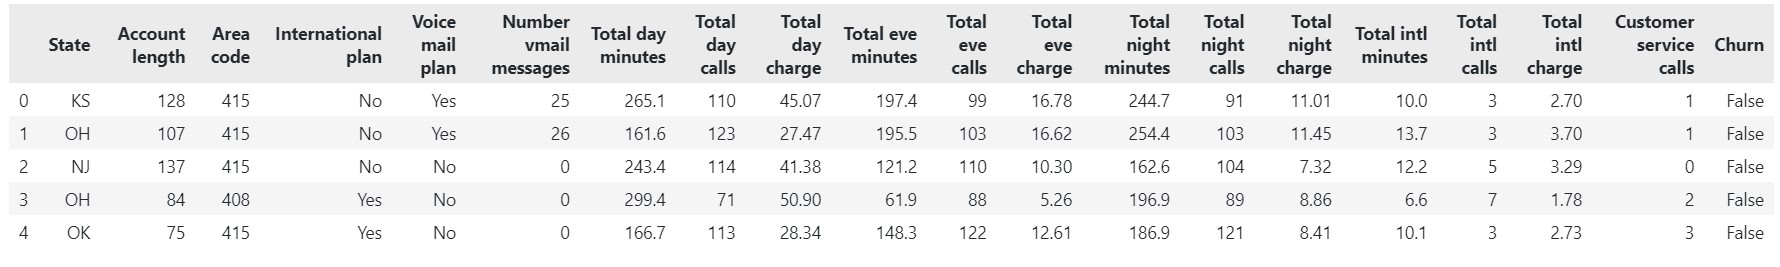
\includegraphics[keepaspectratio,width=500pt]{trainhead.jpg}
    \caption{训练集数据实例}
\end{figure}
\section{对数据属性的理解}
通过上一步我们发现该数据集有$\mathrm{State}$、$\mathrm{Account \enspace length}$、$\mathrm{International\enspace plan}$等
一系列属性,通过查阅相关资料,各属性所包含的意思在下方说明。

$\mathrm{State}$:用户的地区

$\mathrm{Account \enspace length}$:用户账户长度

$\mathrm{Area \enspace code}$:地区代码

$\mathrm{International\enspace plan}$:用户是否订阅国际套餐

$\mathrm{Voice\enspace mail\enspace  plan}$:用户是否开通语音短信

$\mathrm{Number\enspace vmail\enspace messages}$:用户是否开通数字邮件

$\mathrm{Total\enspace day\enspace minutes}$:用户白天通话时长

$\mathrm{Total\enspace day\enspace calls}$:用户白天通话次数

$\mathrm{Total\enspace day\enspace charge}$:用户白天通话话费

$\mathrm{Total\enspace eve\enspace minutes}$:用户傍晚通话时长

$\mathrm{Total\enspace eve\enspace calls}$:用户傍晚通话次数

$\mathrm{Total\enspace eve\enspace charge}$:用户傍晚通话话费

$\mathrm{Total\enspace night\enspace minutes}$:用户夜间通话时长

$\mathrm{Total\enspace night\enspace calls}$:用户夜间通话次数

$\mathrm{Total\enspace night\enspace charge}$:用户夜间通话话费

$\mathrm{Total\enspace intl\enspace minutes}$:用户国际通话时长

$\mathrm{Total\enspace intl\enspace calls}$:用户国际通话次数

$\mathrm{Total\enspace intl\enspace charge}$:用户国际通话话费

$\mathrm{Customer\enspace service\enspace calls}$:用户白天通话时长

$\mathrm{Churn}$:该客户是否流失
\chapter{数据清洗}
\section{查看训练集详细信息}
\begin{lstlisting}
    print(data_train.describe())  
\end{lstlisting}
    \begin{figure}[htbp]
        \centering
        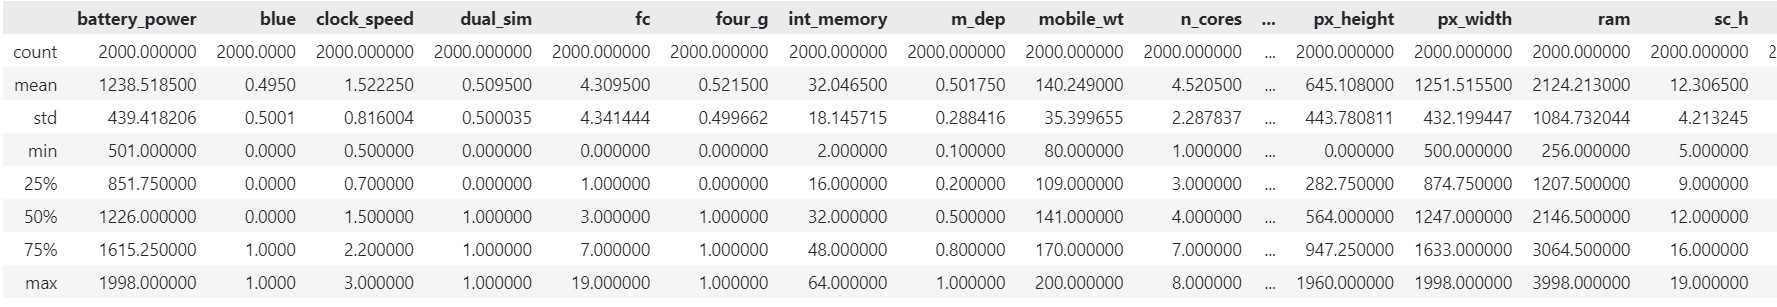
\includegraphics[keepaspectratio,width=400pt]{traindetail.jpg}
        \caption{训练集各数据属性分析}
    \end{figure}
\section{查看数据缺失情况}
\begin{lstlisting}
    print(data_train.info())  
\end{lstlisting}
    \begin{figure}[htbp]
        \centering
        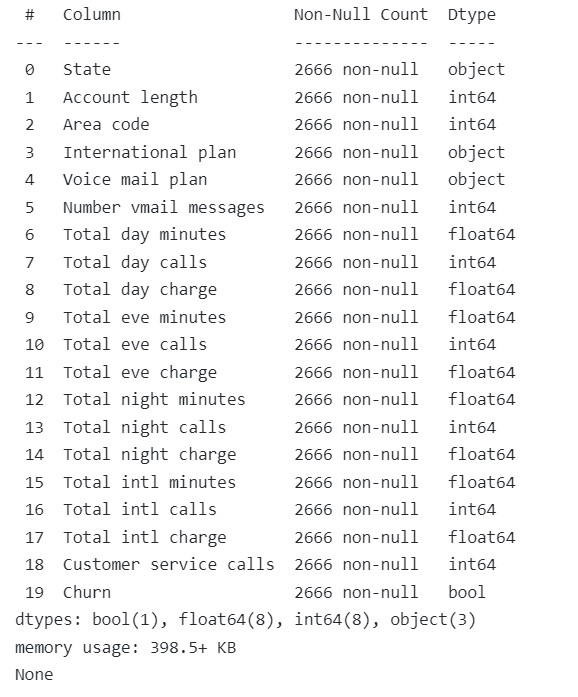
\includegraphics[keepaspectratio,width=400pt]{trainerror.jpg}
        \caption{训练集各数据属性分析}
    \end{figure}
    经观察上图我们发现,各属性数据均完整,下面我们对这些数据进行部分处理。

    \section{数据处理}
    经查阅资料,我们采用以下的代码对数据字符串的部分进行01编码处理。
    \begin{lstlisting}
        # 对数据集中的字符串数据进行编码处理
        gender_class1 = {'No': 0, 'Yes': 1}
        data_train['Voice mail plan'] = data_train['Voice mail plan'].map(gender_class1)
        data_test['Voice mail plan'] = data_test['Voice mail plan'].map(gender_class1)
        gender_class2 = {'No': 0, 'Yes': 1}
        data_train['International plan'] = data_train['International plan'].map(gender_class2)
        data_test['International plan'] = data_test['International plan'].map(gender_class2)
    \end{lstlisting}

    将$\mathrm{Voice\enspace mail\enspace plan}$属性值为No的改为0,属性值为Yes的改为1。

    将$\mathrm{International\enspace plan}$属性值为No的改为0,属性值为Yes的改为1。

\chapter{数据分析}
下面对处理后的数据相关系数热力图进行观察比较,选取我们所需要的对用户是否流失的判断属性。

PS:(由于数据属性过多,这里我们挑选具有代表性的几个属性进行关系分析)
\begin{lstlisting}
    df = data_train[['Voice mail plan','International plan','Account length', 'Area code', 'Number vmail messages', 'Total day minutes', 'Total day calls', 'Total day charge', 'Total eve minutes','Churn']]
    # 属性间相关系数
    cor = df.corr()
    print(cor)
    # 属性间相关系数热力图
    sns.heatmap(cor,cmap="Greens")
    plt.show()
\end{lstlisting}
\begin{figure}[htbp]
    \centering
    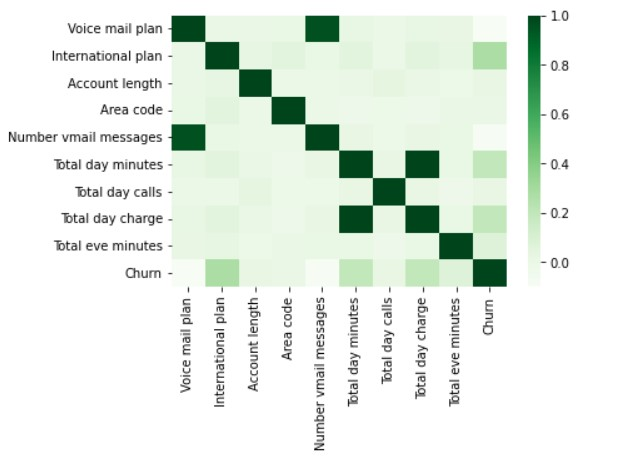
\includegraphics[keepaspectratio,width=460pt]{tconnect.jpg}
    \caption{训练集各数据属性关系分析热力图}
\end{figure}
\begin{figure}[htbp]
    \centering
    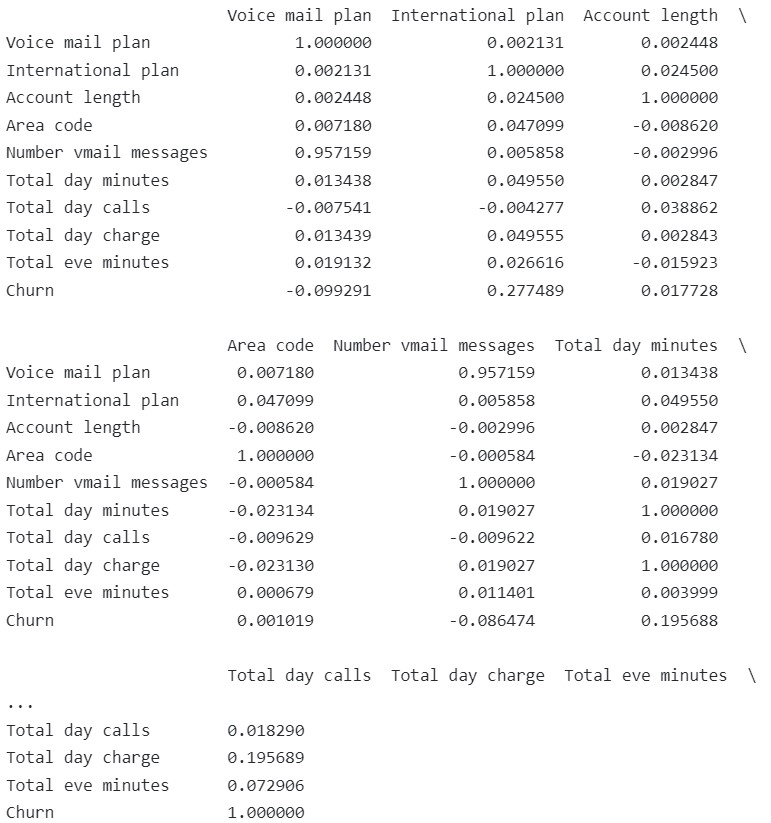
\includegraphics[keepaspectratio,width=400pt]{tconnectlabel.jpg}
    \caption{训练集各数据属性关系分析表}
\end{figure}
通过观察发现,我们发现各属性的相关系数都大致相仿,故我们索性直接将所有属性(不包括$\mathrm{State}$)全部作为训练数据
,送入模型构建中。

\chapter{构建模型及评估}
\section{构建模型前的准备}
我们首先对训练集进行划分,将模型构建的标签和输出(即x和y)准备好。
\begin{lstlisting}
    data_train = data_train.drop(columns=['State'])
    data_test = data_test.drop(columns=['State'])
\end{lstlisting}

首先将无用的$\mathrm{State}$从数据集中去除。

\begin{lstlisting}
    label_train = data_train.loc[:, 'Churn']
    data_train = data_train.drop(columns=['Churn'])
\end{lstlisting}

将$\mathrm{Churn}$作为输出目标,除$\mathrm{Churn}$的以外属性作为判断依据。
\begin{lstlisting}
    train_X=data_train
    train_y=label_train
\end{lstlisting}

将构建模型所需的包导入。
\begin{lstlisting}
    from sklearn.metrics import accuracy_score
    from sklearn.metrics import confusion_matrix
    from sklearn.metrics import precision_score
    from sklearn.metrics import recall_score
\end{lstlisting}
\section{模型构建及评估}

我们分别采用朴素贝叶斯、决策树、多层感知机来进行模型构建,
并分别对模型进行评估。
\subsection{朴素贝叶斯}
\begin{lstlisting}
    # Gaussian Naive Bayes
    from sklearn.naive_bayes import GaussianNB
    
    gaussian = GaussianNB()
    gaussian.fit(train_X, train_y)
\end{lstlisting}
将划分好的数据导入调出模型构建包的函数中,得到模型。
\begin{lstlisting}
    pred_gauss = gaussian.predict(test_X)
    score = gaussian.score(test_X,test_y)
    print(score)
\end{lstlisting}
\begin{figure}[htbp]
    \centering
    
\includegraphics[keepaspectratio,width=300pt]{gaussscore.jpg}
    \caption{朴素贝叶斯模型得分}
\end{figure}
对模型的可行性进行评估。
\begin{lstlisting}
    cm=confusion_matrix(test_y, pred_gauss)
    TP=cm[0,0]
    FP=cm[0,1]
    FN=cm[1,0]
    TN=cm[1,1]
    sns.heatmap(cm,annot=True,cmap='Blues')
    plt.show()
    Accuracy = (TP+TN)/(TP+FP+TN+FN)
    Precision = TP/(TP+FP)
    Recall = TP/(TP+FN)
    print("准确率:",Accuracy)
    print("精准率:",Precision)
    print("召回率:",Recall)
\end{lstlisting}
\begin{figure}[htbp]
    \centering
    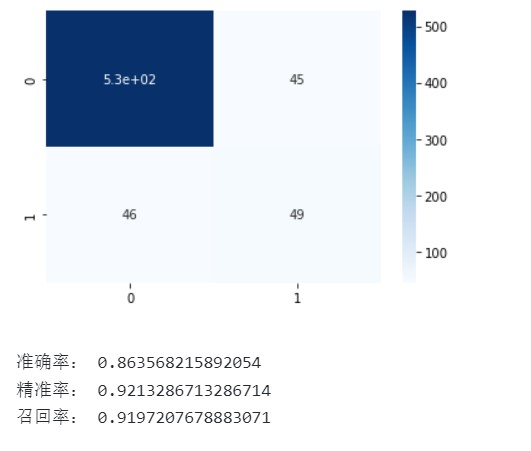
\includegraphics[keepaspectratio,width=300pt]{gauss.jpg}
\end{figure}
依次输出该模型的混淆矩阵、准确率、精准率、召回率。
\subsection{决策树}
\begin{lstlisting}
    #DecisionTree
    from sklearn.tree import DecisionTreeClassifier
    
    decisiontree = DecisionTreeClassifier(max_depth=4)
    decisiontree.fit(train_X, train_y)
\end{lstlisting}
将划分好的数据导入调出模型构建包的函数中,得到模型。
\begin{lstlisting}
    pred_Tree = decisiontree.predict(test_X)
    acc_decisiontree = decisiontree.score(test_X, test_y)
    print(acc_decisiontree)
\end{lstlisting}
\begin{figure}[htbp]
    \centering
    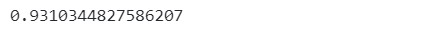
\includegraphics[keepaspectratio,width=300pt]{Treescore.jpg}
    \caption{决策树模型得分}
\end{figure}
对模型的可行性进行评估。
\begin{lstlisting}
    cm=confusion_matrix(test_y, pred_Tree)
    TP=cm[0,0]
    FP=cm[0,1]
    FN=cm[1,0]
    TN=cm[1,1]
    sns.heatmap(cm,annot=True,cmap='Blues')
    plt.show()
    Accuracy = (TP+TN)/(TP+FP+TN+FN)
    Precision = TP/(TP+FP)
    Recall = TP/(TP+FN)
    print("准确率:",Accuracy)
    print("精准率:",Precision)
    print("召回率:",Recall)
\end{lstlisting}
\begin{figure}[htbp]
    \centering
    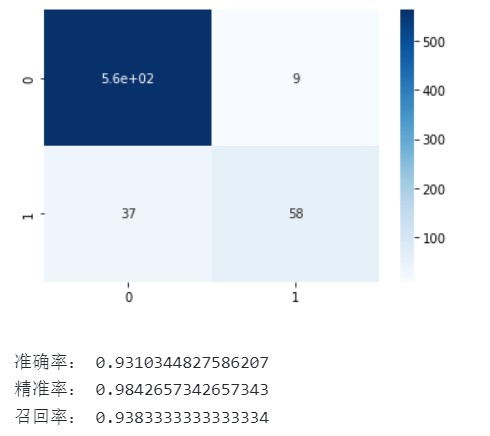
\includegraphics[keepaspectratio,width=300pt]{Tree.jpg}
\end{figure}
依次输出该模型的混淆矩阵、准确率、精准率、召回率。
\subsection{多层感知机}
\begin{lstlisting}
    # MLP
    from sklearn.neural_network import MLPClassifier
    
    mlpc = MLPClassifier(activation='tanh',solver='adam',max_iter=400)
    mlpc.fit(train_X, train_y)
\end{lstlisting}

将划分好的数据导入调出模型构建包的函数中,得到模型。
\begin{lstlisting}
    pred_MLP = mlpc.predict(test_X)
    acc_gbk = mlpc.score(test_X, test_y)
    print(acc_gbk)
\end{lstlisting}
\begin{figure}[htbp]
    \centering
    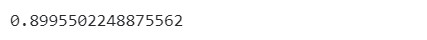
\includegraphics[keepaspectratio,width=300pt]{MLPscore.jpg}
    \caption{多层感知机模型得分}
\end{figure}
对模型的可行性进行评估。
\begin{lstlisting}
    cm=confusion_matrix(test_y, pred_MLP)
    TP=cm[0,0]
    FP=cm[0,1]
    FN=cm[1,0]
    TN=cm[1,1]
    sns.heatmap(cm,annot=True,cmap='Blues')
    plt.show()
    Accuracy = (TP+TN)/(TP+FP+TN+FN)
    Precision = TP/(TP+FP)
    Recall = TP/(TP+FN)
    print("准确率:",Accuracy)
    print("精准率:",Precision)
    print("召回率:",Recall)
\end{lstlisting}
\begin{figure}[htbp]
    \centering
    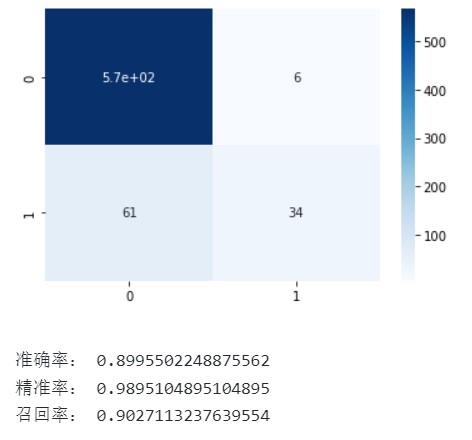
\includegraphics[keepaspectratio,width=300pt]{MLP.jpg}
\end{figure}
依次输出该模型的混淆矩阵、准确率、精准率、召回率。
\chapter{总结与收获}
 
经评估可知各个模型的准确率均高于$80\%$,达到实验预期。
\backmatter


% %=======%
% %引入参考文献文件
% %=======%
\bibdatabase{bib/POC}%bib文件名称 仅修改bib/ 后部分
\printbib
\nocite{*} %显示数据库中有的,但是正文没有引用的文献


% \Appendix

% 这里是附录页,可要可不要

% \Thanks.



\end{document}